\section*{Caso: \( D = 1 \times 10^{-5} \)}


% T = 0
\subsection*{Análise para o caso: \( D = 1 \times 10^{-5} \) e \( t = 0 \)}
A Figura \ref{fig:advec_diffus_1e-05_t0} mostra a distribuição da concentração de soluto no tempo inicial para um coeficiente de difusão \( D = 1 \times 10^{-5} \). Neste caso, observamos que a difusão tem um impacto ainda mais reduzido do que em exemplos anteriores com difusões maiores. A forma retangular inicial praticamente não é alterada, indicando que a advecção domina completamente o transporte do soluto, com a difusão sendo quase negligenciável neste estágio.

\begin{figure}[H]
    \centering
    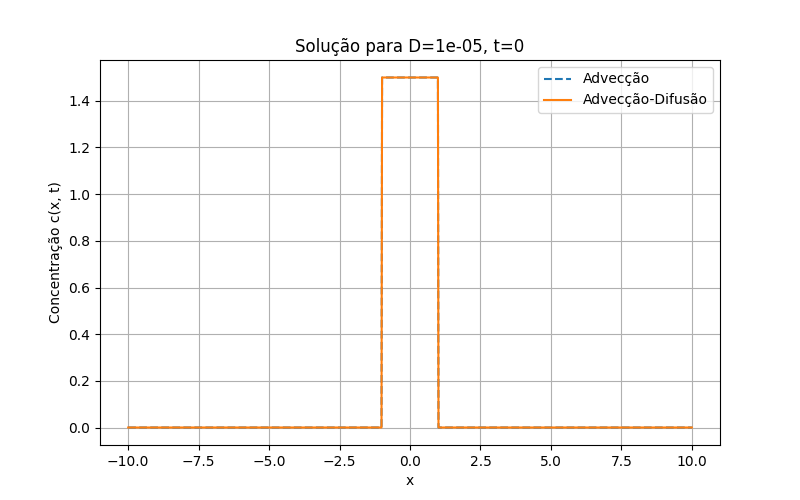
\includegraphics[width=0.7\textwidth]{code/plot/Advec_Difus_t0_D1e-05.png}
    \caption{Comparação das soluções de advecção e advecção-difusão para \( D = 1 \times 10^{-5} \) no tempo \( t = 0 \). A linha tracejada representa a advecção pura, enquanto a linha contínua, quase coincidente com a advecção pura, indica a advecção-difusão.}
    \label{fig:advec_diffus_1e-05_t0}
\end{figure}

\begin{table}[H]
    \centering
    \caption{Valores numéricos da concentração para \( D = 1 \times 10^{-5} \) e \( t = 0 \)}
    \begin{tabular}{ccc}
\toprule
x & Advecção & Advecção-Difusão \\
\midrule
-2.250000 & 0.000000 & 0.000000 \\
-1.690000 & 0.000000 & 0.000000 \\
-1.140000 & 0.000000 & 0.000000 \\
-0.580000 & 1.500000 & 1.500000 \\
-0.030000 & 1.500000 & 1.500000 \\
0.530000 & 1.500000 & 1.500000 \\
1.080000 & 0.000000 & 0.000000 \\
1.640000 & 0.000000 & 0.000000 \\
2.190000 & 0.000000 & 0.000000 \\
2.750000 & 0.000000 & 0.000000 \\
\bottomrule
\end{tabular}

\end{table}


% T = 1
\subsubsection{Análise para o caso: \( D = 1 \times 10^{-5} \) e \( t = 1 \)}

A Figura \ref{fig:advec_diffus_1e-05_t1} mostra a distribuição da concentração de soluto no tempo \( t = 1 \) para um coeficiente de difusão \( D = 1 \times 10^{-5} \). Semelhante ao observado em \( t = 0 \), a difusão tem um efeito ainda muito limitado sobre a distribuição da concentração, que permanece praticamente idêntica à advecção pura. A forma retangular do perfil de concentração persiste sem alterações significativas, demonstrando que, para valores de difusão tão baixos, a difusão não consegue modificar de maneira apreciável a dinâmica imposta pela advecção.

\begin{figure}[H]
    \centering
    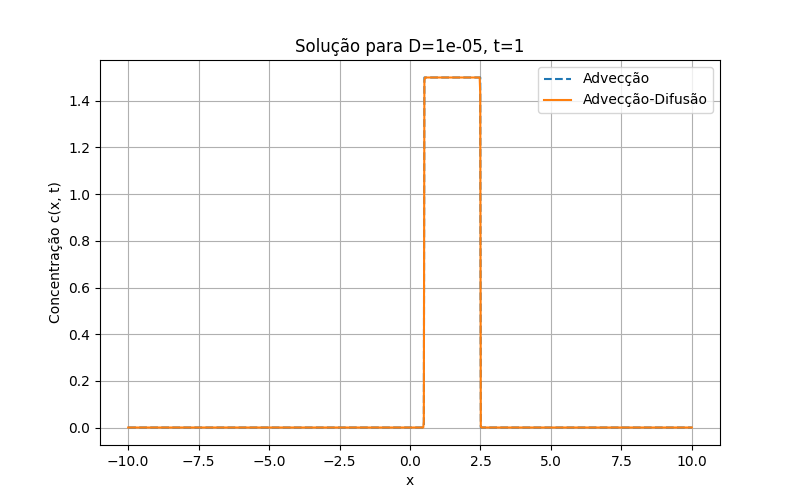
\includegraphics[width=0.7\textwidth]{code/plot/Advec_Difus_t1_D1e-05.png}
    \caption{Comparação das soluções de advecção e advecção-difusão para \( D = 1 \times 10^{-5} \) no tempo \( t = 1 \). A linha tracejada representa a advecção pura, enquanto a linha contínua, quase indistinguível, continua a mostrar o efeito mínimo da difusão.}
    \label{fig:advec_diffus_1e-05_t1}
\end{figure}

\begin{table}[H]
    \centering
    \caption{Valores numéricos da concentração para \( D = 1 \times 10^{-5} \) e \( t = 1 \)}
    \begin{tabular}{ccc}
\toprule
x & Advecção & Advecção-Difusão \\
\midrule
-0.750000 & 0.000000 & 0.000000 \\
-0.190000 & 0.000000 & 0.000000 \\
0.360000 & 0.000000 & 0.000000 \\
0.920000 & 1.500000 & 1.500000 \\
1.470000 & 1.500000 & 1.500000 \\
2.030000 & 1.500000 & 1.500000 \\
2.580000 & 0.000000 & 0.000000 \\
3.140000 & 0.000000 & 0.000000 \\
3.690000 & 0.000000 & 0.000000 \\
4.250000 & 0.000000 & 0.000000 \\
\bottomrule
\end{tabular}

\end{table}



% T = 2
\subsubsection{Análise para o caso: \( D = 1 \times 10^{-5} \) e \( t = 2 \)}

A Figura \ref{fig:advec_diffus_1e-05_t2} mostra a distribuição da concentração de soluto no tempo \( t = 2 \) para um coeficiente de difusão \( D = 1 \times 10^{-5} \). Continuando o padrão observado nos momentos anteriores, a difusão não apresenta um impacto visível na forma da distribuição da concentração, que mantém o perfil retangular. Isso reforça a noção de que, com valores tão baixos de \( D \), a advecção continua sendo a força dominante, com a difusão não proporcionando alterações significativas no transporte do soluto.

\begin{figure}[H]
    \centering
    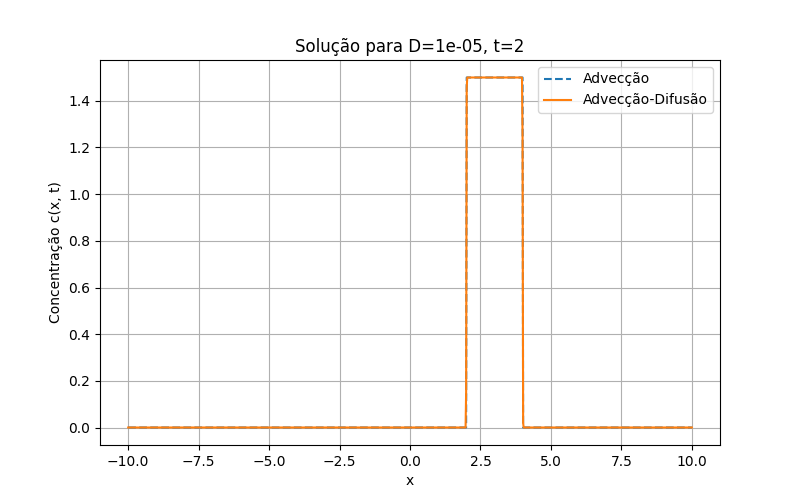
\includegraphics[width=0.7\textwidth]{code/plot/Advec_Difus_t2_D1e-05.png}
    \caption{Comparação das soluções de advecção e advecção-difusão para \( D = 1 \times 10^{-5} \) no tempo \( t = 2 \). A linha tracejada representa a advecção pura, enquanto a linha contínua, quase indistinguível, ilustra o efeito mínimo da difusão.}
    \label{fig:advec_diffus_1e-05_t2}
\end{figure}

\begin{table}[H]
    \centering
    \caption{Valores numéricos da concentração para \( D = 1 \times 10^{-5} \) e \( t = 2 \)}
    \begin{tabular}{ccc}
\toprule
x & Advecção & Advecção-Difusão \\
\midrule
0.750000 & 0.000000 & 0.000000 \\
1.310000 & 0.000000 & 0.000000 \\
1.860000 & 0.000000 & 0.000000 \\
2.420000 & 1.500000 & 1.500000 \\
2.970000 & 1.500000 & 1.500000 \\
3.530000 & 1.500000 & 1.500000 \\
4.080000 & 0.000000 & 0.000000 \\
4.640000 & 0.000000 & 0.000000 \\
5.190000 & 0.000000 & 0.000000 \\
5.750000 & 0.000000 & 0.000000 \\
\bottomrule
\end{tabular}

\end{table}


% T = 3
\subsubsection{Análise para o caso: \( D = 1 \times 10^{-5} \) e \( t = 3 \)}

A Figura \ref{fig:advec_diffus_1e-05_t3} mostra a distribuição da concentração de soluto no tempo \( t = 3 \) para um coeficiente de difusão \( D = 1 \times 10^{-5} \). Assim como nos tempos anteriores, a advecção pura e a advecção-difusão apresentam perfis quase idênticos, com a difusão tendo um impacto ainda inexpressivo sobre a forma da distribuição da concentração. O perfil retangular se mantém praticamente inalterado, reforçando que a advecção domina a dinâmica do transporte do soluto.

\begin{figure}[H]
    \centering
    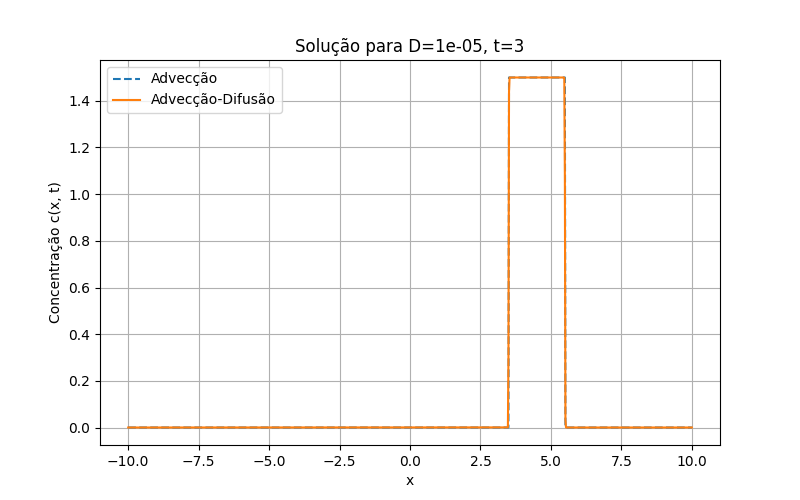
\includegraphics[width=0.7\textwidth]{code/plot/Advec_Difus_t3_D1e-05.png}
    \caption{Comparação das soluções de advecção e advecção-difusão para \( D = 1 \times 10^{-5} \) no tempo \( t = 3 \). A linha tracejada representa a advecção pura, enquanto a linha contínua, ainda quase indistinguível, ilustra o efeito mínimo da difusão.}
    \label{fig:advec_diffus_1e-05_t3}
\end{figure}

\begin{table}[H]
    \centering
    \caption{Valores numéricos da concentração para \( D = 1 \times 10^{-5} \) e \( t = 3 \)}
    \begin{tabular}{ccc}
\toprule
x & Advecção & Advecção-Difusão \\
\midrule
2.250000 & 0.000000 & 0.000000 \\
2.810000 & 0.000000 & 0.000000 \\
3.360000 & 0.000000 & 0.000000 \\
3.920000 & 1.500000 & 1.500000 \\
4.470000 & 1.500000 & 1.500000 \\
5.030000 & 1.500000 & 1.500000 \\
5.580000 & 0.000000 & 0.000000 \\
6.140000 & 0.000000 & 0.000000 \\
6.690000 & 0.000000 & 0.000000 \\
7.250000 & 0.000000 & 0.000000 \\
\bottomrule
\end{tabular}

\end{table}


% T = 4
\subsubsection{Análise para o caso: \( D = 1 \times 10^{-5} \) e \( t = 4 \)}

A Figura \ref{fig:advec_diffus_1e-05_t4} mostra a distribuição da concentração de soluto no tempo \( t = 4 \) para um coeficiente de difusão \( D = 1 \times 10^{-5} \). Continuando com as observações anteriores, a diferença entre a advecção pura e a advecção-difusão é mínima, com a difusão mostrando pouca ou nenhuma capacidade de alterar significativamente o perfil da concentração que permanece quase exclusivamente dominado pela advecção.

\begin{figure}[H]
    \centering
    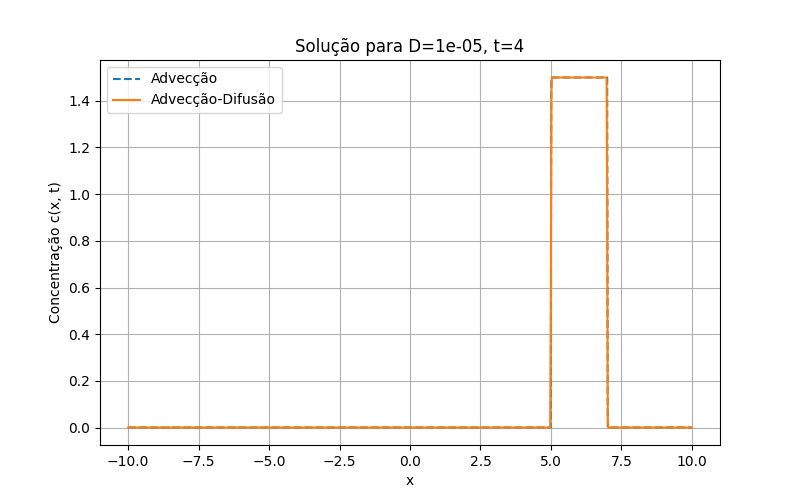
\includegraphics[width=0.7\textwidth]{code/plot/Advec_Difus_t4_D1e-05.png}
    \caption{Comparação das soluções de advecção e advecção-difusão para \( D = 1 \times 10^{-5} \) no tempo \( t = 4 \). A linha tracejada representa a advecção pura, enquanto a linha contínua, quase indistinguível, ilustra o efeito mínimo da difusão.}
    \label{fig:advec_diffus_1e-05_t4}
\end{figure}

\begin{table}[H]
    \centering
    \caption{Valores numéricos da concentração para \( D = 1 \times 10^{-5} \) e \( t = 4 \)}
    \begin{tabular}{ccc}
\toprule
x & Advecção & Advecção-Difusão \\
\midrule
3.750000 & 0.000000 & 0.000000 \\
4.310000 & 0.000000 & 0.000000 \\
4.860000 & 0.000000 & 0.000000 \\
5.420000 & 1.500000 & 1.500000 \\
5.970000 & 1.500000 & 1.500000 \\
6.530000 & 1.500000 & 1.500000 \\
7.080000 & 0.000000 & 0.000000 \\
7.640000 & 0.000000 & 0.000000 \\
8.190000 & 0.000000 & 0.000000 \\
8.750000 & 0.000000 & 0.000000 \\
\bottomrule
\end{tabular}

\end{table}



% T = 5
\subsubsection{Análise para o caso: \( D = 1 \times 10^{-5} \) e \( t = 5 \)}
A Figura \ref{fig:advec_diffus_1e-05_t5} mostra a distribuição da concentração de soluto no tempo \( t = 5 \) para um coeficiente de difusão \( D = 1 \times 10^{-5} \). Consistente com as observações em tempos anteriores, a advecção pura e a advecção-difusão mantêm perfis quase idênticos, com diferenças negligíveis entre eles. Este padrão indica que, mesmo ao longo de um intervalo de tempo estendido, a difusão extremamente baixa não consegue influenciar de maneira significativa a distribuição da concentração, que é amplamente dominada pela advecção.

\begin{figure}[H]
    \centering
    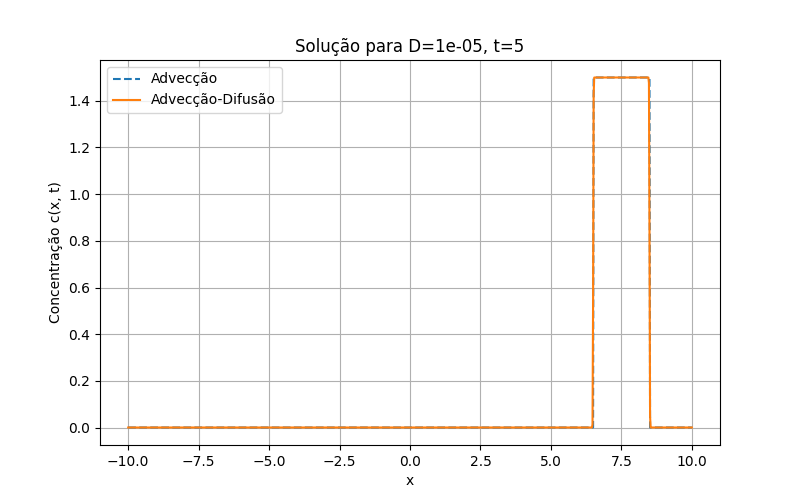
\includegraphics[width=0.7\textwidth]{code/plot/Advec_Difus_t5_D1e-05.png}
    \caption{Comparação das soluções de advecção e advecção-difusão para \( D = 1 \times 10^{-5} \) no tempo \( t = 5 \). A linha tracejada representa a advecção pura, enquanto a linha contínua, quase indistinguível, continua a ilustrar o efeito mínimo da difusão.}
    \label{fig:advec_diffus_1e-05_t5}
\end{figure}

\begin{table}[H]
    \centering
    \caption{Valores numéricos da concentração para \( D = 1 \times 10^{-5} \) e \( t = 5 \)}
    \begin{tabular}{ccc}
\toprule
x & Advecção & Advecção-Difusão \\
\midrule
5.250000 & 0.000000 & 0.000000 \\
5.810000 & 0.000000 & 0.000000 \\
6.360000 & 0.000000 & 0.000000 \\
6.920000 & 1.500000 & 1.500000 \\
7.470000 & 1.500000 & 1.500000 \\
8.030000 & 1.500000 & 1.500000 \\
8.580000 & 0.000000 & 0.000000 \\
9.140000 & 0.000000 & 0.000000 \\
9.690000 & 0.000000 & 0.000000 \\
10.250000 & 0.000000 & 0.000000 \\
\bottomrule
\end{tabular}

\end{table}



% Conclusão do Caso
\subsection*{Conclusão do Caso: \( D = 1 \times 10^{-5} \)}
Durante o período analisado de \( t = 0 \) a \( t = 5 \), as soluções numéricas para a equação de advecção-difusão com um coeficiente de difusão \( D = 1 \times 10^{-5} \) mostraram estabilidade excepcional na distribuição da concentração do soluto. A difusão, neste nível extremamente baixo, demonstrou ter um impacto mínimo, mantendo perfis de concentração quase idênticos aos da advecção pura ao longo de todo o intervalo.

O perfil retangular persistente indica que a difusão é insuficiente para alterar a dinâmica do transporte de soluto, dominada pela advecção. Este caso ressalta que difusões menores são negligenciáveis para mudar a dispersão de solutos em fluxos advectivos, destacando a necessidade de uma parametrização precisa dos modelos de advecção-difusão para representar adequadamente os processos de engenharia e ciências ambientais.
